
% License:
% CC BY-NC-SA 3.0 (http://creativecommons.org/licenses/by-nc-sa/3.0/)
%
%%%%%%%%%%%%%%%%%%%%%%%%%%%%%%%%%%%%%%%%%

%----------------------------------------------------------------------------------------
%	PACKAGES AND OTHER DOCUMENT CONFIGURATIONS
%----------------------------------------------------------------------------------------

\documentclass[paper=a4, fontsize=11pt]{scrartcl} % A4 paper and 11pt font size

\usepackage{listings}
\usepackage{color}

\definecolor{dkgreen}{rgb}{0,0.6,0}
\definecolor{gray}{rgb}{0.5,0.5,0.5}
\definecolor{mauve}{rgb}{0.58,0,0.82}

\lstset{frame=tb,
  language=Java,
  aboveskip=3mm,
  belowskip=3mm,
  showstringspaces=false,
  columns=flexible,
  basicstyle={\small\ttfamily},
  numbers=none,
  numberstyle=\tiny\color{gray},
  keywordstyle=\color{blue},
  commentstyle=\color{dkgreen},
  stringstyle=\color{mauve},
  breaklines=true,
  breakatwhitespace=true,
  tabsize=3
}

\usepackage[T1]{fontenc} % Use 8-bit encoding that has 256 glyphs
\usepackage{fourier} % Use the Adobe Utopia font for the document - comment this line to return to the LaTeX default
\usepackage[english]{babel} % English language/hyphenation
\usepackage{amsmath,amsfonts,amsthm} % Math packages
\usepackage{lipsum} % Used for inserting dummy 'Lorem ipsum' text into the template

\usepackage{caption}
\usepackage{subcaption}
\usepackage{graphicx}

\usepackage{float}

\usepackage{blindtext} %for enumarations

\usepackage[]{hyperref}  %link collor

%talbe layout to the right
%\usepackage[labelfont=bf]{caption}
%\captionsetup[table]{labelsep=space,justification=raggedright,singlelinecheck=off}
%\captionsetup[figure]{labelsep=quad}

\usepackage{sectsty} % Allows customizing section commands
\allsectionsfont{\centering \normalfont\scshape} % Make all sections centered, the default font and small caps

\usepackage{fancyhdr} % Custom headers and footers
\pagestyle{fancyplain} % Makes all pages in the document conform to the custom headers and footers
\fancyhead{} % No page header - if you want one, create it in the same way as the footers below
\fancyfoot[L]{} % Empty left footer
\fancyfoot[C]{} % Empty center footer
\fancyfoot[R]{\thepage} % Page numbering for right footer
\renewcommand{\headrulewidth}{0pt} % Remove header underlines
\renewcommand{\footrulewidth}{0pt} % Remove footer underlines
\setlength{\headheight}{13.6pt} % Customize the height of the header

\numberwithin{equation}{section} % Number equations within sections (i.e. 1.1, 1.2, 2.1, 2.2 instead of 1, 2, 3, 4)
\numberwithin{figure}{section} % Number figures within sections (i.e. 1.1, 1.2, 2.1, 2.2 instead of 1, 2, 3, 4)
\numberwithin{table}{section} % Number tables within sections (i.e. 1.1, 1.2, 2.1, 2.2 instead of 1, 2, 3, 4)

%\setlength\parindent{0pt} % Removes all indentation from paragraphs - comment this line for an assignment with lots of text


\setlength\parskip{4pt}

%----------------------------------------------------------------------------------------
%	TITLE SECTION
%----------------------------------------------------------------------------------------

\newcommand{\horrule}[1]{\rule{\linewidth}{#1}} % Create horizontal rule command with 1 argument of height

\title{	
\normalfont \normalsize 
\textsc{Innopolis University} \\ [25pt] % Your university, school and/or department name(s)
\horrule{0.5pt} \\[0.4cm] % Thin top horizontal rule
\huge  Differential Equations \\ Computational Practicum - Task 14 \\ $y' = (1 + \frac{y}{x}) \ln \frac{x+y}{x} + \frac{y}{x}$\\ % The assignment title
\horrule{2pt} \\[0.5cm] % Thick bottom horizontal rule
}

\author{Trang Nguyen} % Your name

\date{\normalsize\today} % Today's date or a custom date

\begin{document}
%\nocite{*}
\maketitle % Print the title

\newpage
\begin{abstract}

Consider the initial value problem with the ODE of the first order and some interval:
$$\left\lbrace \begin{array}{ll} y'=f(x,y) \\ y(x_0)=y_0 \\ x\in [x_0, X] \end{array}\right.$$

In this document, I will analyze a specific problem (task 14) where $f(x,y)=(1 + \frac{y}{x}) \ln \frac{x+y}{x} + \frac{y}{x}$, $x_0=1$, $y_0=2$ and $X=6$. The exact solution and it's corresponding approximations in three numerical methods, i.e. Euler's method, improved Euler method and Runge-Kutta method will be implemented in a Java application. This application also provides data visualization; and allows user to change initial value $x_0$, $y_0$, $X$ and grid size hence ability to compare methods.

The overview of the problem and methods will be presented in the first part. Following is about implementation in Java. Finally, analysis using implemented application will be provided.
    
\end{abstract}

\section{Solution}
\label{chapter1}

Consider the initial value problem with the ODE of the first order and some interval:
$$\left\lbrace \begin{array}{ll} y'=f(x,y)=(1 + \frac{y}{x}) \ln \frac{x+y}{x} + \frac{y}{x} \\ y(x_0)=y_0 \\ x\in [x_0, X] \end{array}\right.$$

Obviously, $f(x,y)$ is defined when $x\neq 0$ and $\frac{x+y}{x} > 0$

\subsection{Exact solution}

Let $r = \frac{y}{x}$, $y'=(1+\frac{y}{x}\ln \frac{x+y}{x} + \frac{y}{x}$ becomes: $r'x+r=(1+r)\ln (1+r) + r$

$$\Rightarrow \frac{dr}{(1+r)\ln (1+r)}=\frac{dr}{x}$$

$$\Rightarrow \int_{\frac{y_0}{x_0}}^{r} \frac{dr}{(1+r)\ln (1+r)} = \int_{x_0}^{x}\frac{dx}{x}$$

$$\Rightarrow \ln \frac{\ln (1+r)}{\ln (1+\frac{y_0}{x_0}} = \ln \frac{x}{x_0}$$

$$\Rightarrow y = x(1+\frac{y_0}{x_0}^\frac{x}{x_0} - x$$

Therefore, $y=x(1+\frac{y_0}{x_0}^\frac{x}{x_0}-x$ where $x\neq 0$ and $\frac{x+y}{x} > 0$ is the exact solution of $y'=(1+\frac{y}{x})\ln \frac{x+y}{x} + \frac{y}{x}$

\subsection{Numerical Methods}

We are interested in computing approximate values of solutions of $y'=f(x,y)$, $y(x_0)=y_0$ at equally spaced points $x_0, x_1,..,x_n=X$ in an interval $[x_0, X]$. 
$$x_i = x_0 + ih, i = 0, 1,...,n \text{ where } h=\frac{X-x_0}{n}$$

Local error (error at the $i$th step): $e_i = y(x_i)-y_i$

Global error: $e = e_n = y(X)-y_n$

\subsubsection{Euler Method}

Euler method is the simplest numerical method which is based on the assumption that the tangent line at $(x_i, y(x_i)$ approximate the integral curve over $[x_i, x_{i+1}]$. It starts with the known value $y(x_0) = x_0$ and computes $y_1, y_2,...,y_n$ by the formula:

$$y_{i+1} = y_i + hf(x_i, y_i) \text{ , }0\leq i\leq n-1$$

\subsubsection{Improved Euler Method}

The improved Euler method starts with the known value $y(x_0) = x_0$ and computes $y_1, y_2,...,y_n$ by the formula:

$$k_{1i} = f(x_i, y_i)$$
$$k_{2i} = f(x_i + h, y_i + hk_{1i})$$
$$y_{i+1} = y_i + \frac{h}{2}(k_{1i} + k_{2i})$$

\subsubsection{Runge-Kutta Method}

Runge-Kutta is the most widely method. It starts with the known value $y(x_0) = x_0$ and computes $y_1, y_2,...,y_n$ by the formula:

$$k_{1i} = f(x_i, y_i)$$
$$k_{2i} = f(x_i + \frac{h}{2}, y_i + \frac{h}{2}k_{1i})$$
$$k_{3i} = f(x_i + \frac{h}{2}, y_i + \frac{h}{2}k_{2i})$$
$$k_{4i} = f(x_i + h, y_i + hk_{3i}$$
$$y_{i+1} = y_i + \frac{h}{6}(k_{1i} + 2k_{2i} + 2k_{3i} + k_{4i})$$


\section{Java application}
\label{chapter2}

Above solutions are implemented in Java using Netbeans and SceneBuilder. This application provides GUI which allows user to alter $x_0$, $y_0$, $X$ and grid size $n$ in constraint, i.e. $x_0, X \neq 0$, $\frac{x_0+y_0}{x_0} > 0$ (to ensure that $f(x,y)$ is defined) and $X > x_0$, $n\in N$, $n > 0$. Since $f(x,y)$ is not defined at $x=0$, for the ease of implementation, I applied one more constraint to user input: $x_0$ and $X$ must have the same sign (both positive or both negative).

\subsection{User guide}

\textbf{Highlight features}
\begin{itemize}  
\item Allow changing initial values $x_0$, $y_0$, $X$ and grid size $N$.
\item Allow choosing methods: exact solution, Euler method, improved Euler method and Runge-Kutta method.
\item Provide visualization for solutions, local errors and global errors for chosen methods.
\end{itemize}

\begin{figure}[H]
	\centering
	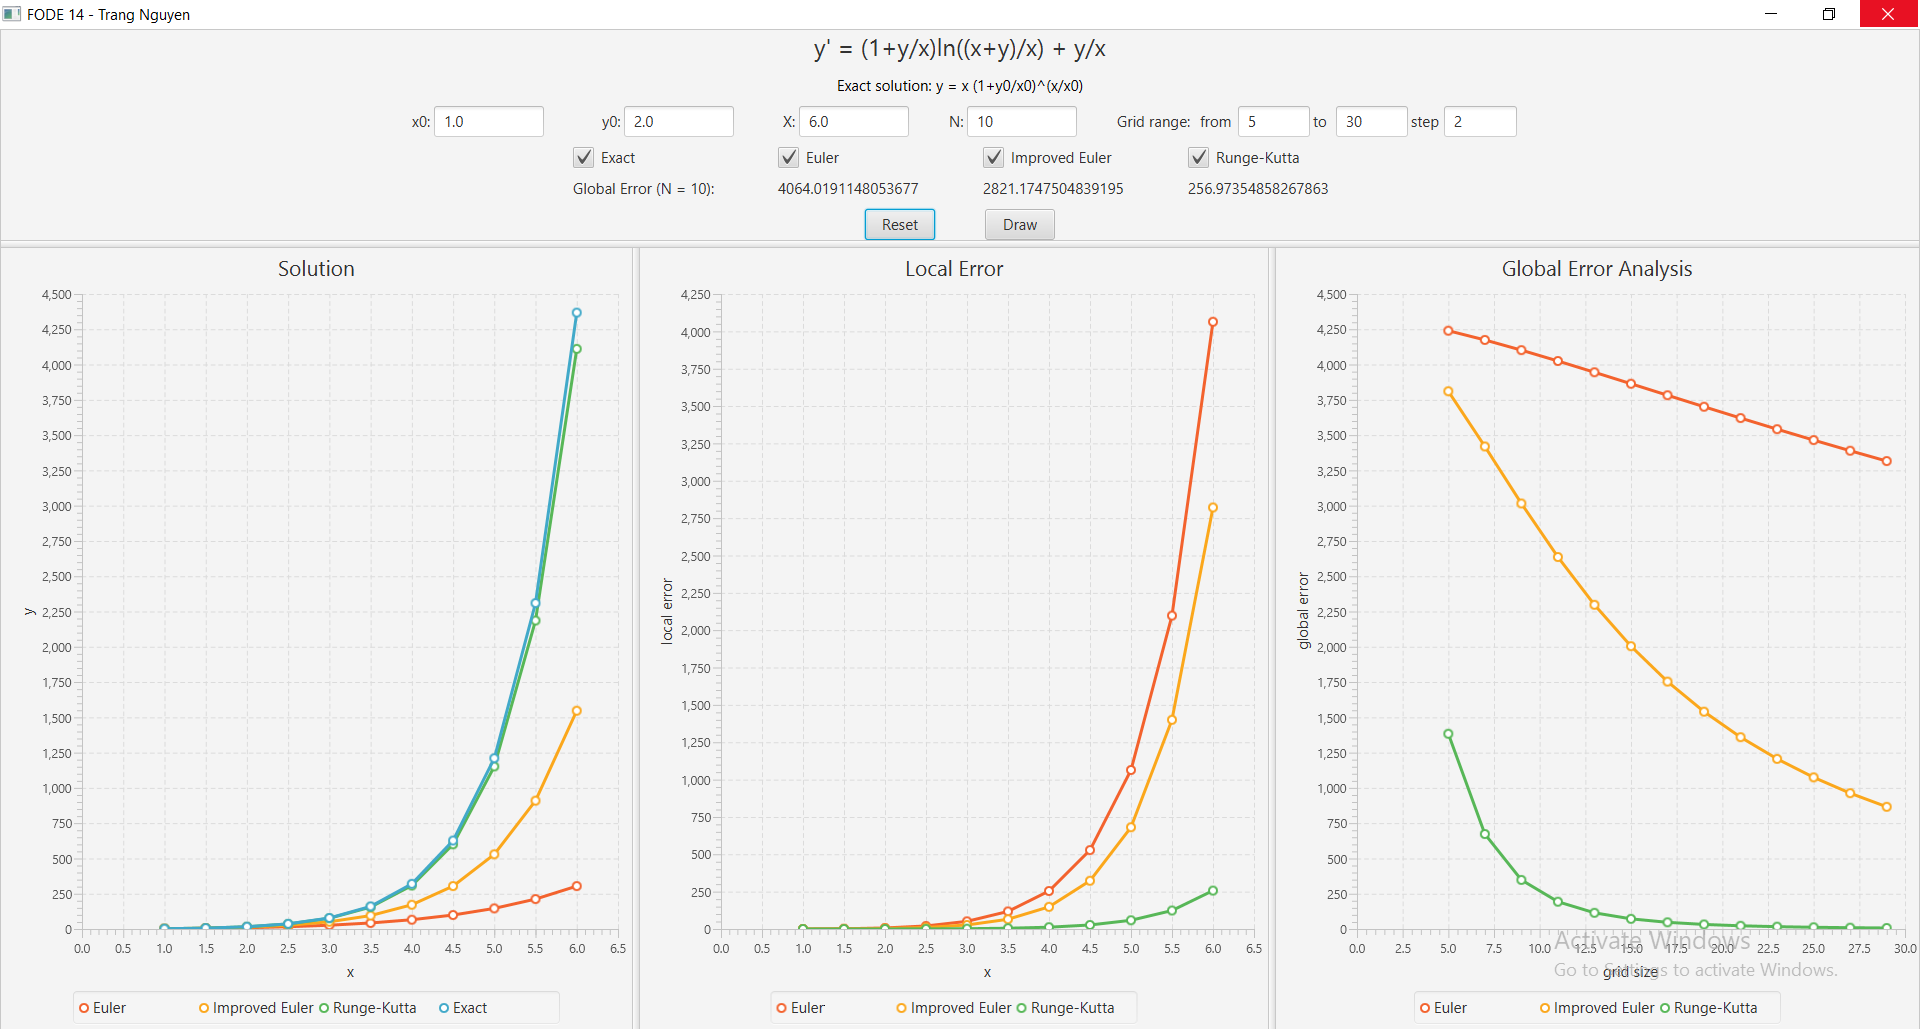
\includegraphics[width=\linewidth]{image/full.png}
	\caption{Application screenshot with default values}
	\label{fig:applicationscreenshot}
\end{figure}

\textbf{How to use}
\begin{enumerate}  
\item Enter valid initial values $x_0$, $y_0$, and $X$, grid size $N$ and grid range. Default values: $x_0=1.0$, $y_0=2.0$, $X=6.0$, $N=10$ and grid range from 5 to 30 with step of 2. Any invalid input will be informed.
\begin{figure}[H]
	\centering
	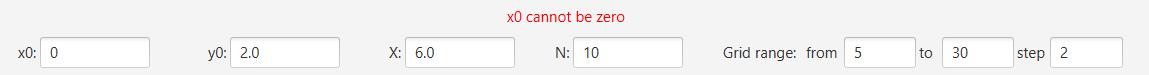
\includegraphics[width=0.8\linewidth]{image/error.png}
	\caption{Enter values}
	\label{fig:entervalues}
\end{figure}
\item Choose methods to process. Both Exact, Euler, Improved Euler and Runge-Kutta are chosen by default.
\begin{figure}[H]
	\centering
	
\includegraphics[width=0.8\linewidth]{image/method.png}
	\caption{Choose methods}
	\label{fig:choosemethods}
\end{figure}
\item Click 
\includegraphics[height=2\fontcharht\font`\B]{image/draw.png} button to start analyzing. \\Global errors with specified $N$ will be presented right below chosen methods.
\begin{figure}[H]
	\centering
	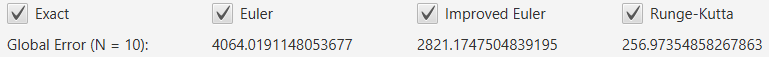
\includegraphics[width=0.8\linewidth]{image/global.png}
	\caption{Global Errors at $N$}
	\label{fig:globalerror}
\end{figure}
Also, plots of solutions, local errors, global errors in grid range will be updated in drawing space.
\begin{figure}[H]
	\centering
	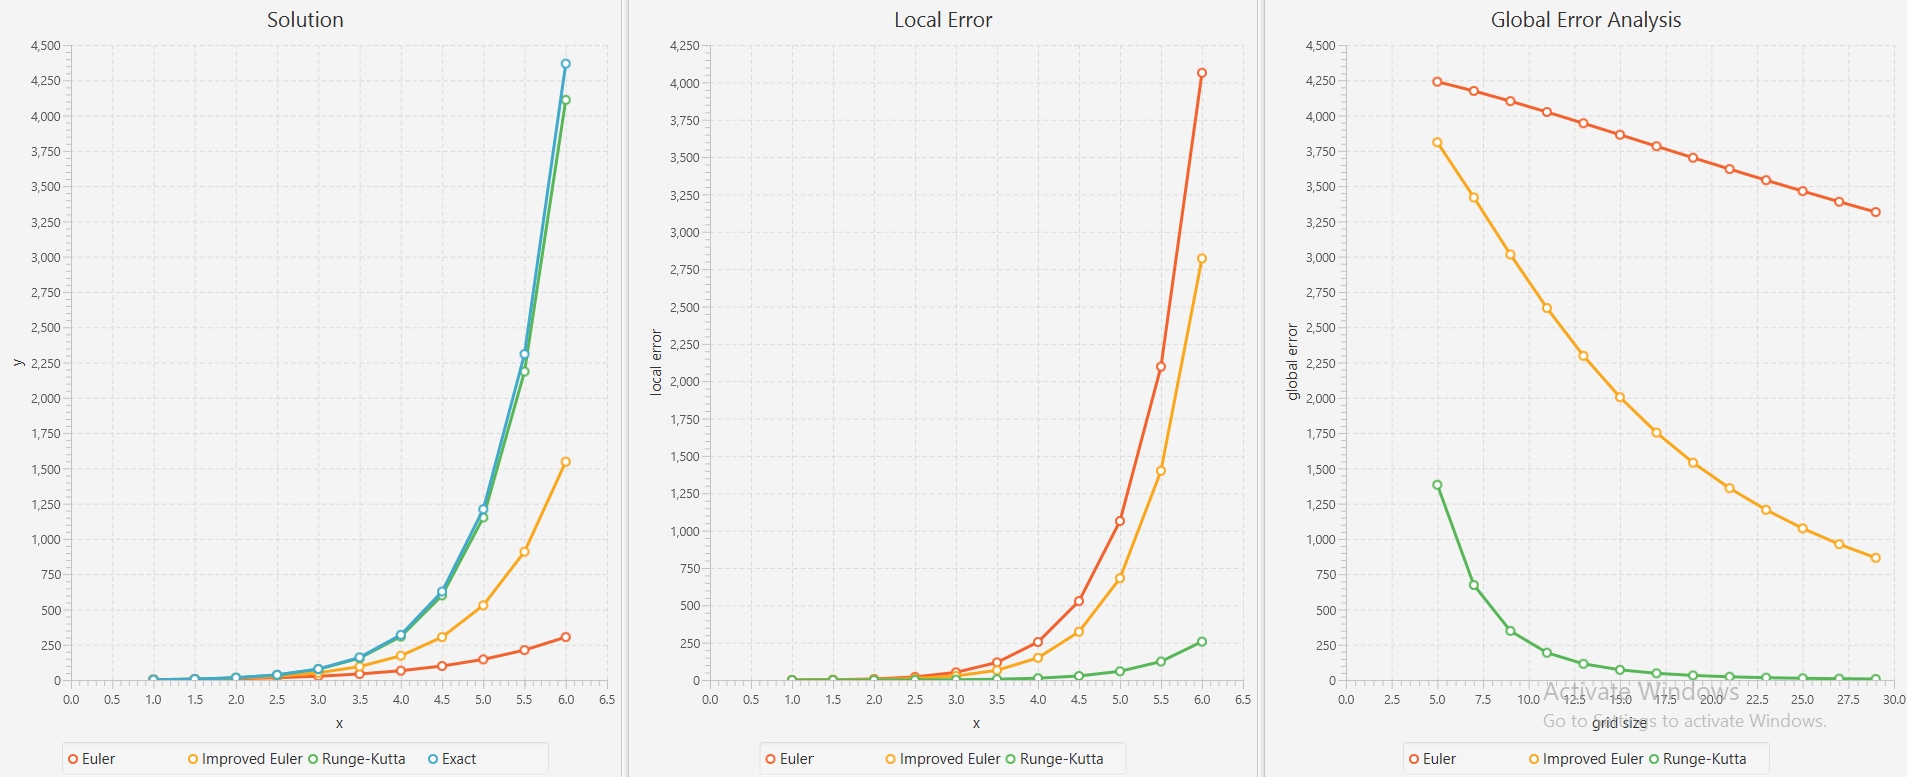
\includegraphics[width=\linewidth]{image/plot.png}
	\caption{Plots of solutions, local errors at $N$; and global errors in grid range}
	\label{fig:plot}
\end{figure}

\end{enumerate}
Click 
\includegraphics[height=2\fontcharht\font`\B]{image/reset.png} button to reset all elements to default values.

\subsection{Implementation}

The application is written in Java using Netbeans and SceneBuilder. Since for each initial value $x_0$, and $y_0$; and $X$, exact solution and it's approximation should be provided, I decided to used only one class named Fode14 for our ODE. In GUI, there is only two event handlers (for clicking "Draw" and "Reset" buttons) which are in FXMLDocumentController class.

\begin{figure}[H]
	\centering
	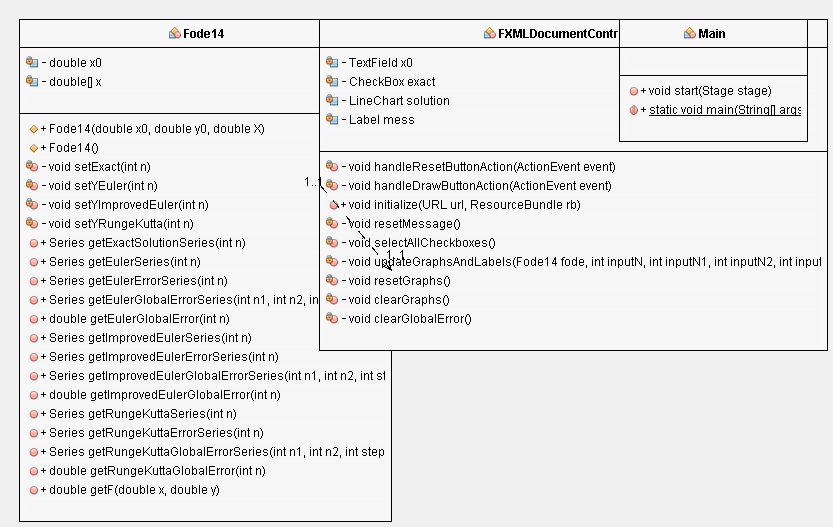
\includegraphics[width=\linewidth]{image/uml.png}
	\caption{UML Diagram}
	\label{fig:uml}
\end{figure}

Below is implementation of Runge-Kutta method (as functions in Fode14). It's structure is applicable for others.
\begin{lstlisting}
    private void setYRungeKutta(int n) throws Exception {
        setExact(n);
        
        if (yRungeKutta == null || yRungeKutta.length != n+1) {
            yRungeKutta = new double[n+1];
            yRungeKutta[0] = y0;

            double k1, k2, k3, k4;
            double h = (X-x0)/n;
            for (int i = 0; i < n; ++i) {
                k1 = getF(x[i], yRungeKutta[i]);
                k2 = getF(x[i] + h/2.0, yRungeKutta[i] + h*k1/2.0);
                k3 = getF(x[i] + h/2.0, yRungeKutta[i] + h*k2/2.0);
                k4 = getF(x[i] + h, yRungeKutta[i] + h*k3);
                yRungeKutta[i+1] = yRungeKutta[i] + h*(k1+2*k2+2*k3+k4)/6.0;
            }
        }
    }
    
    public Series getRungeKuttaSeries(int n) throws Exception {
        Series rungeKutta = new Series();
        rungeKutta.setName("Runge-Kutta");
        
        setYRungeKutta(n);
        for (int i = 0; i <= n; ++i) {
            rungeKutta.getData().add(new XYChart.Data(x[i], yRungeKutta[i]));
        }
        return rungeKutta;
    }
    
    public Series getRungeKuttaErrorSeries(int n) throws Exception {
        Series rungeKutta = new Series();
        rungeKutta.setName("Runge-Kutta");
        
        setYRungeKutta(n);
        for (int i = 0; i <= n; ++i) {
            rungeKutta.getData().add(new XYChart.Data(x[i], yExact[i] - yRungeKutta[i]));
        }
        return rungeKutta;
    }
    
    public Series getRungeKuttaGlobalErrorSeries(int n1, int n2, int step) throws Exception {
        if (n1 <= 0 || n2 <= 0 || n1 >= n2 || step <= 0) {
            throw new Exception("Invalid Grid range input");
        }
        Series rungeKutta = new Series();
        rungeKutta.setName("Runge-Kutta");
        
        for (int i = n1; i <= n2; i += step) {
            rungeKutta.getData().add(new XYChart.Data(i, getRungeKuttaGlobalError(i)));
        }
        
        return rungeKutta;
    }
    
    public double getRungeKuttaGlobalError(int n) throws Exception {
        setYRungeKutta(n);
        return yExact[n] - yRungeKutta[n];
    }
\end{lstlisting}

\section{Analysis}
\label{chapter3}

\begin{figure}[H]
	\centering
	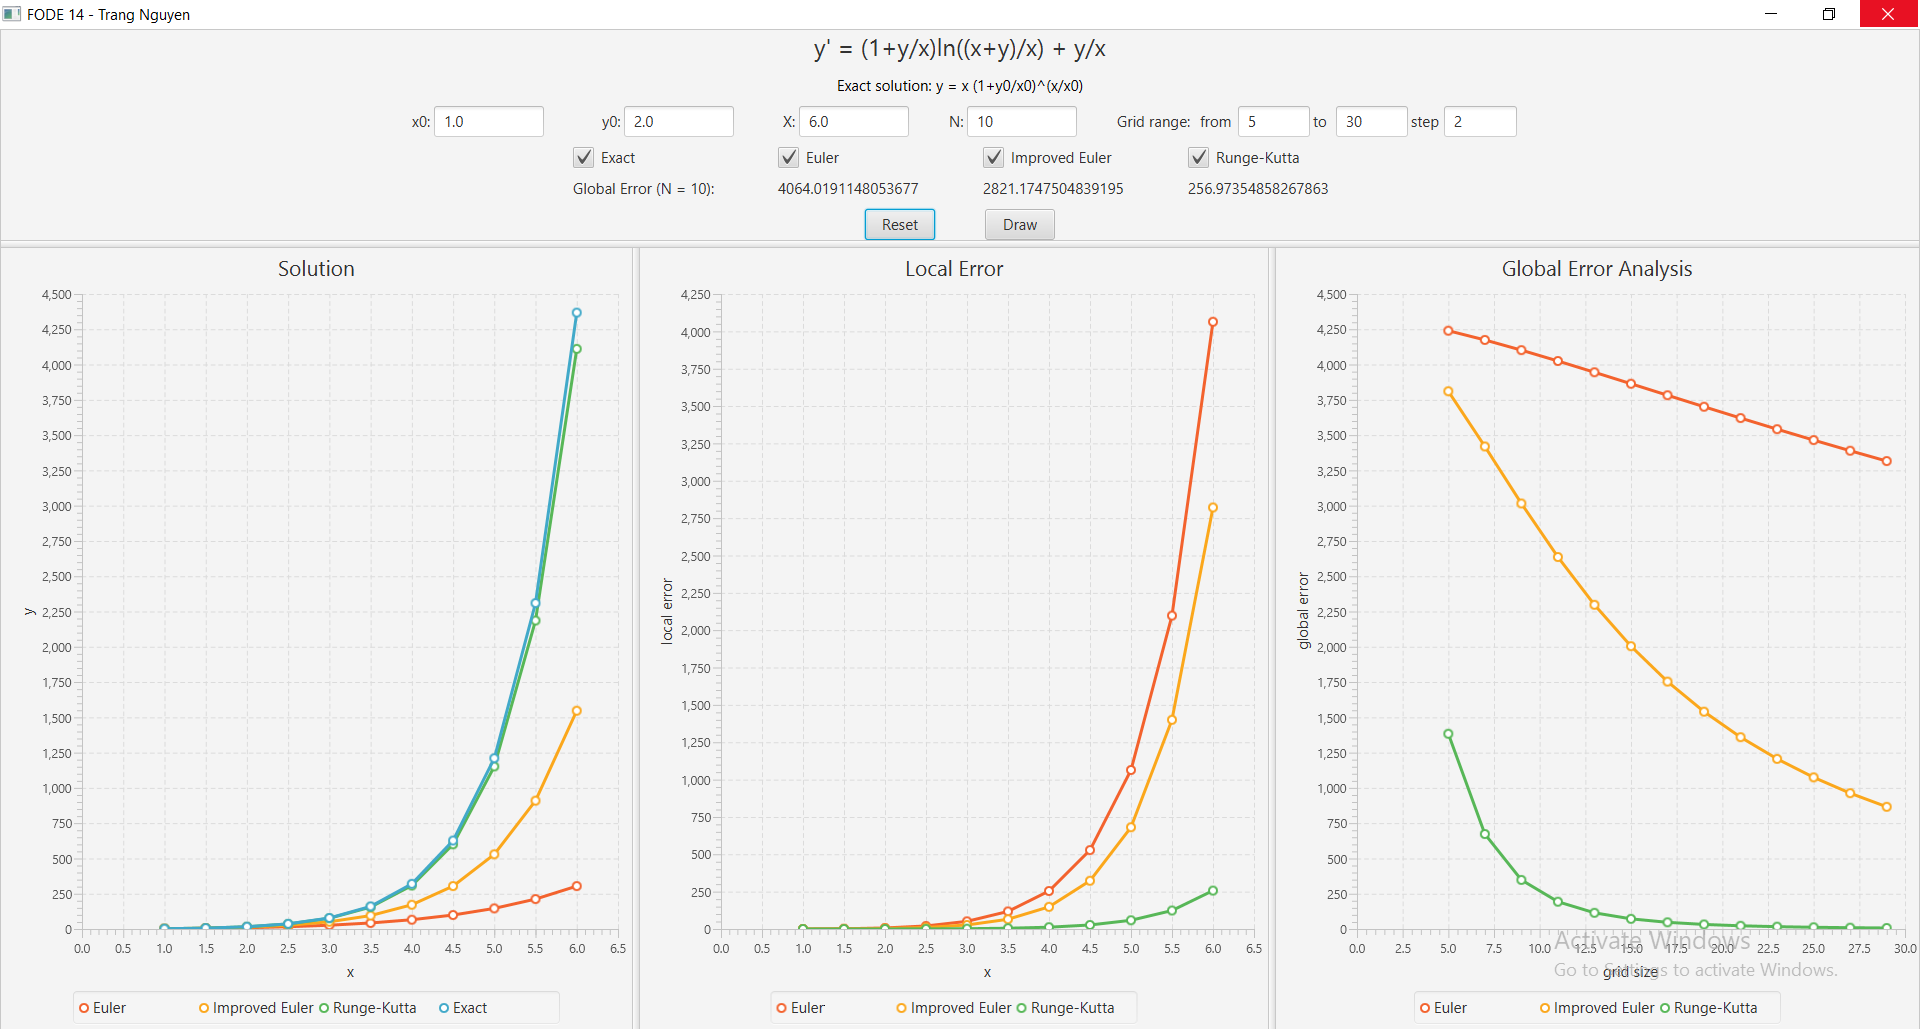
\includegraphics[width=\linewidth]{image/full.png}
	\caption{Analysis with $x_0=0.1$, $y_0=2$, $X=6.0$, $N=10$, grid range = $(5,30,2)$}
	\label{fig:applicationscreenshot}
\end{figure}

Analyzing using the software, we can infer that:
\begin{itemize}  
\item Runge-Kutta method has the highest performance (closest to exact solution, lowest local and global errors). Following is Improved Euler, and Euler method.
\item For $x_0=0.1$, $y_0=2$, $X=6.0$, from $N=20$, increasing $N$ does not significantly affect accuracy of Runge-Kutta method. This number for improved Euler method is around 150, and for Euler method is around 2000.
\end{itemize}

\end{document}